\chapter{Integrating the simulator into Kubernetes}

Batsim is able to run simulations of any distributed system, to study any
event-based scheduler that would implement its message protocol. Kubernetes is
a piece of software where all its component, including the scheduler, revolve
around a central API. Everything is asynchronous as the API can be
accessed anytime by any component.

The question that arises is, can we adapt Batsim to make it support Kubernetes
schedulers? Is it possible to implement an adaptive layer between a synchronous
event based simulator like Batsim and a scheduler implemented following the
asynchronous paradigms of APIs? To answer these issues we developed
Batkube\footnote{github.com/oar-team/batkube}, which is an adaptive interface
to Batsim for Kubernetes schedulers.

It will follow that in order to do so, we re-implemented an API following
Kubernetes specifications and intercepted the scheduler's time to synchronize
it with the simulation time. This allows us to simulate lengthy workloads in a
short period using a scheduler otherwise supposed to rely on ``real'' machine
time. We first describe some technical concepts about Kubernetes and Batsim,
and then describe how we re-implemented the API, intercepted the time, and
handled the synchronization of the different times between Batsim and the
scheduler.

\section{Batsim concepts}

A Batsim simulation is divided into two processes: Batsim itself and the
decision process (the scheduler).  As a consequence, Batsim defines its own
messaging protocol to be able to standardize exchanges with the scheduler. This
protocol takes the form of a text based interface that conveys the events
occuring during the simulation.

\begin{figure}[H]
	\centering
	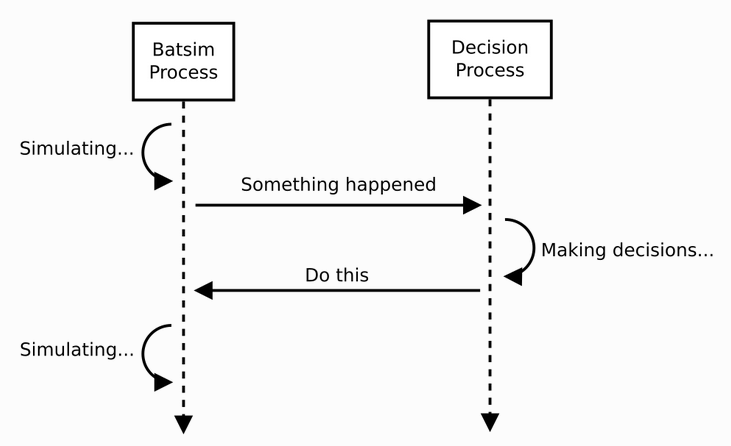
\includegraphics[scale=0.5]{imgs/batsim-sequence-diag.png}
	\captionsource{Exchanges between Batsim and the scheduler.}{https://batsim.readthedocs.io/en/latest/protocol.html}
	\label{fig:bati-seq-diag}
\end{figure}

A Batsim platform is a SimGrid platform, defined in the xml format. A node can
endorse the role of \textit{master}, \textit{compute\_resource} or
\textit{storage}. Here we only consider master nodes which host the decision
process, and compute resources to which we add our custom resource capacities.
These additional fields are \textit{core}\footnote{The core field is already
present in the resource definition, but it is not forwarded to Batsim for
unknown reasons at the time this report is written.} which is the amount of cpu
the node has and \textit{memory} which is memory capacity of the node. Of
course, storage resources can be taken into account in future development of
Batkube. Also, we do not consider the links between the nodes for now because
we do not support parallel jobs. Finally, Batsim proposes an energy model that
we decided to ignore as well.\\

Batsim takes one or several workload as inputs, which are json files containing
jobs definitions. Figure \ref{fig:bat_wl_ex} gives an example of such workload.
The jobs are defined with the following inputs.  First, they are identified by
an \textit{id} which is unique within each workload and are submitted at a time
defined by the \textit{subtime} field. The \textit{res} field states the number
of resources each job requires, although we don't use this field because we
can't specify \textit{which} resource we require. Instead we pass resource
requests as optional parameters. We support the additional fields \textit{cpu}
which has a minimum value of 100m cpu just like Kubernetes cpu
requests\footnote{https://kubernetes.io/docs/concepts/configuration/manage-resources-containers/}
and \textit{memory} which also complies with Kubernetes compute resource
definitions.  Jobs follow a certain \textit{profile} that defines the nature of
the job.  These profile may be as simplistic as \textit{delay} profile which
makes the resource wait for a given amount of time, or describe parallel tasks
using matrices to describe the amount of exchanges between the allocated nodes.
For now we only consider delays to simplify the implementation of the
simulator. Also, because Kubernetes allows the use of multiple
schedulers\footnote{https://kubernetes.io/docs/tasks/extend-kubernetes/configure-multiple-schedulers/},
we support the field \textit{scheduler} which contains the name of the
scheduler the job should be scheduled with.\\

Batsim messaging interface is based on its protocol. Each message is composed
of the field \textit{timestamp} which contains the current simulation time, as
well the field \textit{events} which is a list of events either from Batsim to
the scheduler, or from the scheduler to Batsim. Figure \ref{fig:batmsg_ex}
depicts a standard message sent from the scheduler to Batsim.  Batkube features
are limited because we focused on building a working proof of concept rather
than a fully fledged Kubernetes simulator which is why only consider a subset
of these messages. We provide a list of supported events and their description
in the section \ref{batmsg} of the appendix. More information on Batsim's
protocol is available on Batsim
documentation\footnote{https://batsim.readthedocs.io/en/latest/protocol.html}

Batsim's output takes the form of a csv file containg information about the
jobs executions. Mainly we take interest in their submission time, execution
time and waiting time. Again, a detailed list of Batsim outputs can be found on
the
documentation\footnote{https://batsim.readthedocs.io/en/latest/output-jobs.html}.
During our experimentations with Batkube we interest ourselves in two metrics
that can be computed from this output:
\begin{itemize}
	\item The \textit{makespan}, which is the total length of the
		simulation. It is defined as the timestamp at which the last
		job finishes executing, minus the origin (in this case, zero).
	\item The \textit{mean\_waiting\_time}, which is the mean time the jobs
		spent waiting for a scheduling decision. The waiting time is
		defined by the duration between the submission time and the
		starting time (here the starting time is equivalent to the time
		at which the job was scheduled. We will see later that these
		two times do not correspond in Kubernetes.)
\end{itemize}

These metrics were chosen because in our case, they are representative of the
accuracy of the simulation. Time synchronization (see section
\ref{sec:time-hijack}) may introduce delays in the scheduling decision, thus
increasing the overall makespan and mean waiting time of the simulation.
%Experiments showed that the makespan does not vary much from simulation to
%simulation, but due to Batkube simulations stochastic nature the decisions
%taken by the scheduler may vary from experiment to experiment, thus introducing
%variations in the mean waiting time.

\section{Kubernetes concepts}

Kubernetes is now a large ecosystem to which more than 2 700 developers have
contributed over the years. In this section we present the fundamental concepts
and the components that make up Kubernetes.

\begin{figure}[h]
	\centering
	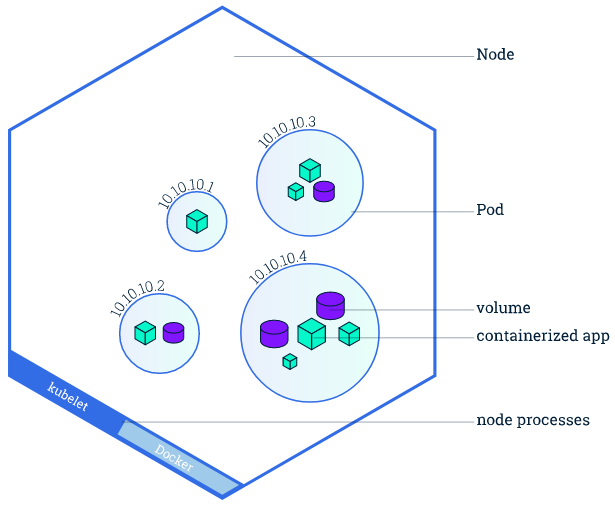
\includegraphics[scale=0.5]{./imgs/node-overview.png}
	\captionsource{Node overview}{https://kubernetes.io/docs/tutorials/kubernetes-basics/explore/explore-intro/}
	\label{fig:node-overview}
\end{figure}

The basic processing unit of Kubernetes is called a \textbf{pod} which is
composed of one or several containers and volumes\footnote{Because of their
	transient nature, containers can not store data on their own. A volume
	is some storage space on the host machine that can be linked to
containers, in order for them to read and write persistent information.}. The
type of application they contain vary depending on the context: in a web
platform context a pod most often hosts a service or micro-service that must be
available at all times, in opposition to a batch processing context where it
runs an application that is to be executed in a finite amount of time.  Pods
are bundled together in \textbf{nodes} (figure \ref{fig:node-overview}) which
are either physical or virtual machines. They represent another barrier to pass
through to access the outside world which bundles pods under the same network
to facilitate communication between them, and enables the use of proxies to
access the underlying services. A set of nodes is called a \textbf{cluster}
which is the highest abstraction layer in Kubernetes.

Nodes take the idea of containerization further than plain containers by
encapsulating the already encapsulated services.  Each node runs at least one
pod, the \textbf{kubelet}, which is a process responsible for communicating
with the rest of Kubernetes. More precisely, the kubelet communicates with the
\textbf{kube-api-server} which is responsible for the whole cluster. We refer
to this API as the api-server, as it is called within the Kubernetes community.
This API server, as well as the other components of the \textbf{Control Plane}
(figure \ref{fig:kube-components}), can be run on any machine but for
simplicity they are set up on the same machine at start up. This machine is
often called the \textbf{master} node and typically does not run any other
container.

As stated before Kubernetes revolves around its API server which is its central
component. All operations between components go through this REST API. These
operations take various forms like user interactions through the commande line
interface \textbf{kubectl}, scheduling operations or management of cluster data
on \textbf{etcd}. We then decided to re-build the API in order to simulate any
cluster to -- almost -- any Kubernetes scheduler.

TODO: Talk about Kubernetes schedulers. What they are based on, how they communicate to Kubernetes.

\begin{figure}[h]
	\centering
	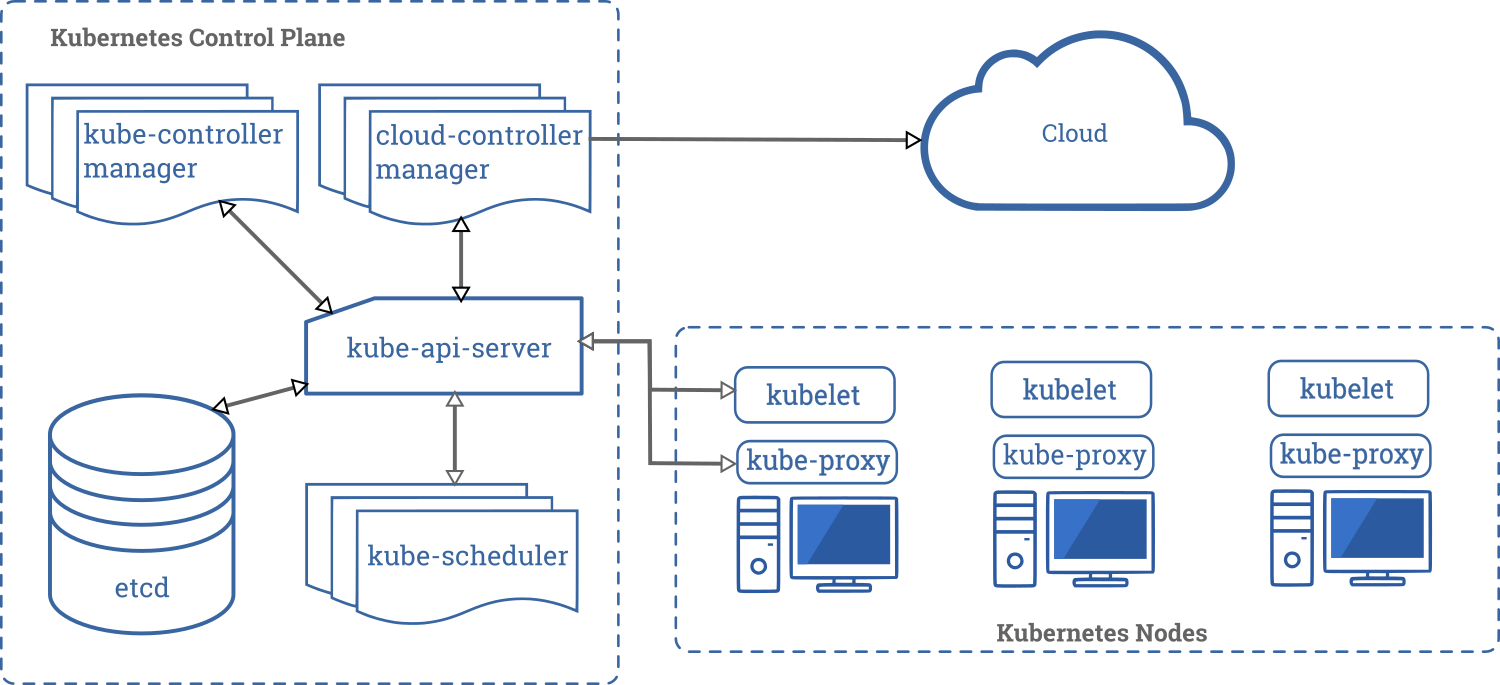
\includegraphics[width=\textwidth]{./imgs/components-of-kubernetes.png}
	\captionsource{Components of Kubernetes}{https://kubernetes.io/docs/concepts/overview/components/}
	\label{fig:kube-components}
\end{figure}

\section{General architecture of Batkube and its integration with Kubernetes and Batsim}

\subsection{Integration with Kubernetes}

In order to adapt Kubernetes schedulers for use with Batsim we need to position
ourselves between the Kubernetes scheduler and the cluster. Several level of
implementations are possible, and after some considerations described in
section \ref{sec:imp_levels} of the appendix we decided to reimplement
Kubernetes API. This new implementation will act as a Kubernetes cluster to the
scheduler, and as an event based scheduler to Batsim.

\begin{figure}[h]
	\centering
	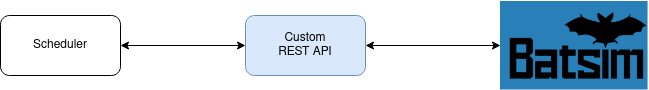
\includegraphics[width=\textwidth]{imgs/custom-restapi.png}
	\caption{Custom REST API in between the scheduler and Batsim.}
	\label{fig:custom-api}
\end{figure}

Building a new API allows us to consider only the endpoints we need and have
complete control over the source code. The technically challenging aspect here
is Kubernetes resource management. Indeed, we need to provide the scheduler
with expected informations about the cluster state if we want to obtain a
correct behavior from it, and while the endpoints of the API are well
documented, Kubernetes team did not write lengths about how resources are
managed internally. In order to save us the hassle of writing the entire code
of the server, we used tools to generate the code from the api-server
specification as described in section \ref{sec:api}.

\subsection{Architecture of Batkube}

Figure \ref{fig:batkube-architecture} depicts the architecture of Batkube,
which is written in Go.  The central component is the \textbf{broker}. It
handles the messages coming from Batsim and the scheduler while ensuring time
synchronization between them. It is responsible for translating and forwarding
messages between Batsim and the scheduler and orchestrates the synchronization
between the two parties.  \textbf{batsky-go} intercepts the calls to Go
\textit{time} library to ensure the scheduler's time is based on the simulation
time instead of machine time. Time requests are forwarded to Batkube which
replies with the current simulation time.  The complete process to ``hijack''
scheduler time is explained in section \ref{sec:time-hijack}. The \textbf{rest
api} is the reimplementation of the Kubernetes api-server. It ensures the
scheduler gets all the necessary information on the cluster state to make its
scheduling decisions, and it is also the receiver of those decisions. Section
\ref{sec:api} explains how we built this API and a tool to automatically
generate its code from the api-server specification.  \textbf{translate} is a
utility package providing functions to translate Kubernetes resources to Batsim
messages, and \textit{vice versa}.

\begin{figure}[h]
	\centering
	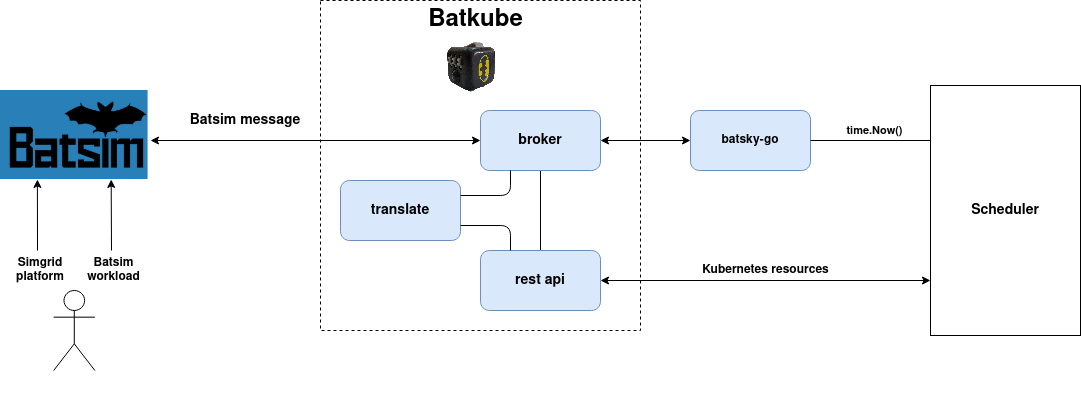
\includegraphics[width=\textwidth]{imgs/batkube-architecture-3-synchro.png}
	\caption{Architecture of Batkube}
	\label{fig:batkube-architecture}
\end{figure}

\section{Building the API} \label{sec:api}

The API of Kubernetes follows the
OpenAPI\footnote{https://www.openapis.org/about} 2 specification which is a
standard for describing APIs. Luckily tools exist to generate such
specification from source code, but also to generate code from a specification.
Since the Kubernetes API specification is available on their
reposotory\footnote{https://github.com/kubernetes/kubernetes/blob/release-1.18/api/openapi-spec/swagger.json},
we were able to use such tools. This allowed us not to implement boiler plate
code by hand and fill the gaps where they needed to be filled, leaving empty
the endpoints we do not need. These endpoints can be dealt with later for
future development of the simulator. For this project we used
go-swagger\footnote{https://github.com/go-swagger/go-swagger/tree/master/examples/stream-server}
to generate our code and the API specification corresponds to the release 1.18
of Kubernetes. One downside of this method is that go-swagger forbids to tamper
with the code of the server itself, although we did not need to during this
project.\\

In order to enable communication between Batsim and the scheduler we need to
translate Batsim messages into Kubernetes resources that can be retrieved by
the scheduler and scheduler decisions to Batsim messages. Batsim Jobs are
simply translated to pods. Jobs do exist in Kubernetes, but they are simply
wrappers around pods: when submitting a job to the (real) api-server, the api
ensures that a pod is created and executed to completion. In our case, we do
not need such intermediate. Compute resources are simply translated to
Kubernetes nodes.

\section{Time interception} \label{sec:time-hijack}

Kubernetes schedulers are not event based schedulers. They constantly check on
the cluster state and make decisions accordingly, therefore they are based on
machine time to make their decisions. However, in order to have correct
simulations, the scheduler needs to be synchronized with simulation time. We
then need to intercept all calls to machine time to redirect them to the
simulator. There are two approaches to this: either we patch the C library used
by Go (figure \ref{fig:patch-C}) and compile Go using our library, or we patch
Go's time library (\ref{fig:patch-go}) and then patch the scheduler so it uses
our library instead of the official one.

Using this tool we patched the
kube-scheduler\footnote{https://github.com/kubernetes/kube-scheduler}, that we
used during our experiments, and also the
kube-batch\footnote{https://github.com/kubernetes-sigs/kube-batch} scheduler.
The latterreceived the patch without any issues, but we couldn't use it because
it implied more development on the batkube api to support it.

\begin{figure}[]
	\centering
	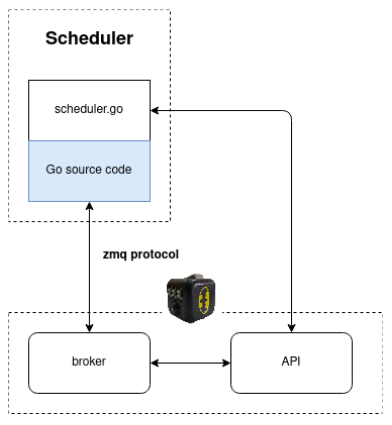
\includegraphics[scale=0.75]{imgs/time-hijack-Go.png}
	\caption{Partially reimplementing Go source code allow us to intercept calls to get machine time.}
	\label{fig:patch-time}
\end{figure}

\subsection{Redirection of time requests to Batkube}

The module in charge of this time redirection is called
\textbf{batsky-go}\footnote{https://github.com/oar-team/batsky-go}, which re
implements \texttt{time.Now()} as well as timers and tickers. Timers are
structures that are instantiated with a duration as input, that notify the
caller once this duration is elapsed. Timers can be reset, modified or deleted
after initialization, which make their implementation tricky in a parallel
computing context. Tickers are essentially the same structures as timers,
except they regularly notify the caller with the given period of time instead
of exiting after they fire like timers would.

In order to explain batsky-go algorithms as clearly as possible we need to
provide some context about Go channels. Go allows the user to run multi
threaded code easily thanks to its \textbf{go routines}. These routines allow
the user to run code in parallel whithout requiring any setup by simply calling
\texttt{go func()} where \texttt{func()} is a function.  It creates a new
thread and launches the given code in parallel with the encapsulating function.
Essentially, this creates a child process.  Go \textit{channels} are
\textit{``a typed conduit through which you can send and receive values with
the channel operator, <-''}\footnote{source:
https://tour.golang.org/concurrency/2}

\begin{figure}[]
	\begin{minted}{go}
ch <- v    // Send v to channel ch.
v := <-ch  // Receive from ch, and
           // assign value to v.
   \end{minted}
   \caption{Usage of a Go channel}
   \label{fig:go-channel}
\end{figure}

A channel can be shared amongst several process and allow several pieces of
code run in parallel to share data, without having to implement any mutex. By
default sends and receives on a channel are blocking operations. If the two
lines from figure \ref{fig:go-channel} were to be executed one after the other,
the program would remain stuck on the first line, as it would wait for some
process to receive the data sent on \texttt{ch} which only happens on the
second line.\\

\SetKwInput{KwInput}{Input}
\SetKwInput{KwOutput}{Output}

\begin{algorithm}[]
\DontPrintSemicolon
\KwResult{Current simulation time}
\KwInput{req: requests channel, resMap: response channel map}
\KwOutput{now : simulation time}

\If{requester loop is not running}{
	go runRequesterLoop() \tcc{There can only be one loop runing at a time}
}
id = newUUID()\;
res = newChannel()\;
resMap[id] = res \tcc{A channel is associated with each request}
req $<$- id \tcc{The code blocks here until request is handled}
now = $<$-res \tcc{The code blocks here until response is sent by the requester loop}
return now\;
\caption{Time request (time.now())}
\label{alg:now}
\end{algorithm}

Let us call \texttt{time.Now()} calls \textit{time requests}. Channels enable
us to centralize time requests from multiple simultaneous callers in one place
before forwarding all requests to Batkube. There are two parts to
\texttt{batsky-go}. One is composed of the many requesters, and the other one
is the loop centralizing requests and handling exchanges with Batkube which we
will call ``the main loop''.  Figure \ref{alg:now} gives the new implementation
of time.Now(), which is the ``requester'' part. Each request is identified
using a unique id to keep track of the pending requests that are waiting for a
response. \texttt{resMap} is a thread safe channel map that is shared amongst
the requesters and the main loop containing (id, response channel) key-value
pairs. When a new request is made, a new entry is created on this map and the
requester will wait for a response on the newly created channel, associated
with its id. All requests are sent to a unique channel \texttt{req}. To make a
new request, the requester simply sends its id to this channel.

\begin{algorithm}[]
\DontPrintSemicolon
\KwInput{req: requests channel, resMap: response channel map}
\While{Batkube is not ready} {
	wait\;
}
requests = []request\;
\While{req is not empty} {
	id = $<$- req \tcc{Non blocking receive}
	requests = append(requests, id)\;
}
now = getCurrentTimeFromBatkube()\;
\For{m in requests} {
	resMap[id] $<$-now \tcc{The caller resumes execution upon reception}
}

\caption{Requester loop}
\label{alg:reqLoop}
\end{algorithm}

Each iteration of the main loop first waits for a signal from Batkube
indicating that the broker is ready to handle the time request. That way, we
make sure we don't miss out on any request because the requests accumulate on
the \texttt{req} channel in the mean time, while minimizing potential downtime
because we know Batkube will answer instantly. Once we get the signal that
Batkube is ready all is left to do is retrieve the ids from our requesters,
retrieve the time from the simulation, and answer each individual request.
Figure \ref{fig:time-interception} presents a typical exchange between the
scheduler, batsky-go and Batkube.

\begin{figure}[]
	\centering
	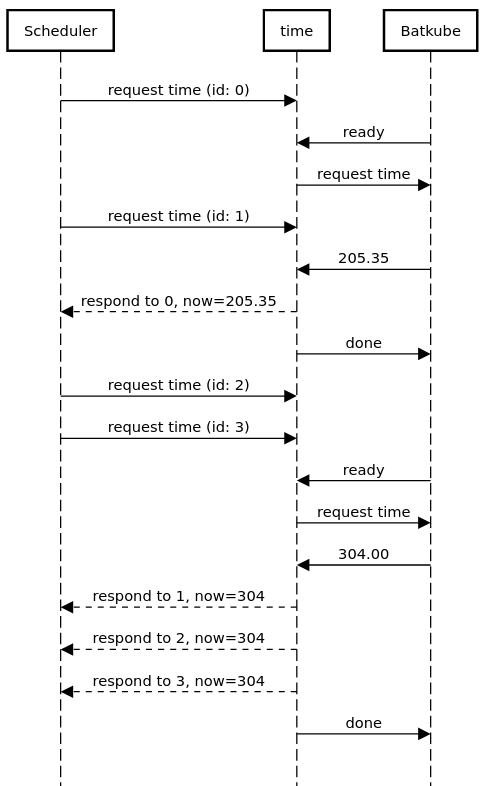
\includegraphics[scale=0.43]{imgs/requester_broker_no_CML.png}
	\caption{Exchange breakdown between batsky-go and Batkube.}
	\label{fig:time-interception}
\end{figure}

\subsection{Patching schedulers} \label{sec:patch-scheds}

We have developed a tool for patching the schedulers, so they use our library
instead of the standard \texttt{time} library. This tool is called
\texttt{batsky-go-installer} and is available on github alongside
Batkube\footnote{github.com/oar-team/batsky-go-installer}.

Our approach replaces all calls to the functions of the \texttt{time} library
while leaving the objects as is to ensure compatibility. In that regard, our
approach makes use of standard \texttt{time} objects instead of redefining new
custom objects, which would break compatibility with the rest of the code. It
makes use of Go Abstract Syntax Tree (AST) to go through the source files and
replace the appropriate symbols, while adding the import to our module whenever
it is necessary. Go \texttt{ast} package make it very convenient to search and
replace symbols in the syntax tree.  Unfortunately, we cannot replace the calls
of the Go source code itself with this approach which creates inconsistencies
between the scheduler code now based on simulation time, and native Go code
still based on machine time. Aside from creating warnings, these
inconsistencies did not prevent the scheduler to function correctly.

\section{Time synchronization}

Synchronization of the time between the scheduler and the simulator is the
critical part of Batkube, because this is where we make compromises between the
speed and the accuracy of the simulation. The scheduler is not event-based and
therefore we can never know for sure when it will send a decision. Therefore we
need to listen to the scheduler as much as we can, but while we do so the
simulation advances slowly. In fact, whenever we listen to the scheduler and
wait for a decision we synchronize machine time and simulation time so the
scheduler gets a time that advances as it would if it was not simulated. This
ensures that the internals of the scheduler function correctly. We could speed
up this time to increase simulation speed and study the effect it has on the
scheduler, but we have to leave this for future work unfortunately. During that
time Batsim is blocked and waits for a message from the decision process. When
we give back priority to Batsim time stops advancing on the scheduler side,
effectively suspending the decision process. At this time Batsim advances
forward in the simulation and replies with new events. Figure
\ref{fig:time_sync} gives a breakdown of the exchanges between Batsim, Batkube
and the scheduler with their associated times.\\

\begin{figure}[]
	\centering
	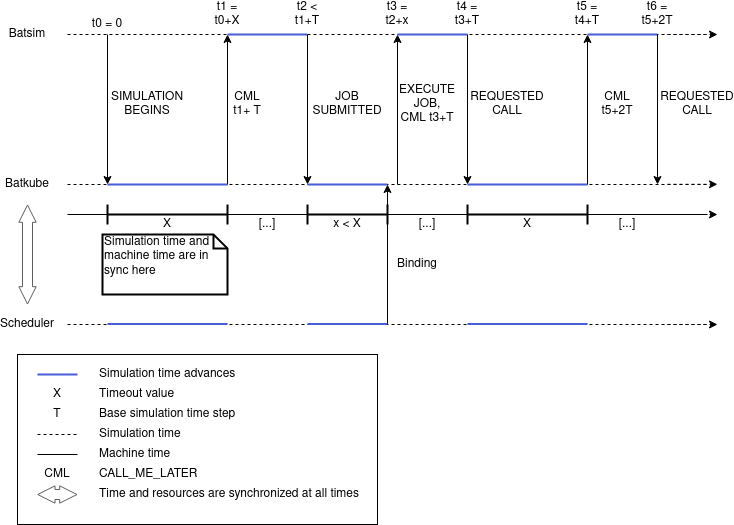
\includegraphics[width=0.8\textwidth]{imgs/lignes_de_temps.png}
	\caption{Time sync between the three components. The broker has to take
	into account both machine time and simulation time.}
	\label{fig:time_sync}
\end{figure}

The simulator can be tuned with several parameters which have various effect on
the simulation. We study those effects in section \ref{sec:params-eval}.

\begin{itemize}[leftmargin=*]
	\item To limit the time we spend waiting for the scheduler we
		implemented a timeout policy. The \textit{timeout value}
		defines the maximum amount of time we spend waiting for a
		scheduler decision: after this amount of time we get back to
		Batsim to go forward in the simulation. Whenever we receive a
		decision from the scheduler, we immediately give back control
		to Batsim by sending it the decision. 
	\item Also, we added the \textit{minimum delay} parameter, which is
		analogous to \textit{timeout value}. It defines the minimum
		amount of time we remain in Batkube each cycle: we will always
		wait at least this amount of time for the scheduler even though
		we already received a scheduling decision. This parameter was
		implemented because we observed incorrect behavior of the
		scheduler -- it crashed -- when Batkube responded too quickly.
		However, this issue seems resolved with latest updates of the
		Kubernetes scheduler and it seems we don't need this mechanic
		anymore. It might still be useful for other schedulers or
		earlier versions of the kube-scheduler which is why we keep it
		in the simulator.
	\item Whenever we block the scheduler to send a message to Batsim, the
		latter supposedly advances the simulation as far as it desires.
		This may impact the decision process because we can't know for
		sure if the scheduler would have made a decision in the mean
		time. If that is the case, this decision will be drastically
		delayed or canceled. This is why we only allow Batsim to jump
		forward in time up to a certain \textit{simulation timestep}.
		This time step varies between \textit{base-simulation-timestep}
		and \textit{max-simulation-timestep}: it starts at the base
		timestep and increases following a backoff policy. This policy
		is implemented as follow: the time step is multiplied by a
		factor every time the scheduler did not provide any decision,
		and reset when we receive a decision from the scheduler. This
		ensures Batsim does not jump to much forward in time while
		increasing simulation speed when the scheduler does not have
		any decision to make. We tell Batsim to ``wake up'' at certain
		times thanks to CALL\_ME\_LATER (CML) events. When Batsim
		receives such events, it replies with a REQUESTED\_CALL at the
		timestamp specified in the CML event.
	\item To speed up the simulation in its last steps, we implemented a
		parameter allowing Batsim to jump forward in time as much as
		desired when no jobs or in \textit{pending} state, that is to
		say waiting to be scheduled. We allow such behavior when the
		scheduler is not supposed to make any decision when no jobs are
		to be scheduled, which is the case with the kube-scheduler.
		This would lead to incorrect simulations with more advanced
		schedulers implementing features such as \textit{preemption},
		which allows schedulers to kill running jobs in order to make
		room for large jobs, to resume the jobs that were killed later.
		This improves the overall makespan of the simulation.
	\item To improve the experiments stability we implemented a feature to
		detect scheduler crashes. Despite all our efforts at making
		simulation as stable as possible, simulated time still causes
		some crashes on the scheduler side. We detect such crashes and
		exit Bakube with an error code when it happens. A crash is
		detected when the scheduler had to make a decision but did not
		react for some time (that we can configure, independently of
		the \textit{timeout value}). We consider that the scheduler has
		to make a decision when no jobs are running and some jobs are
		pending, waiting for a decision.
\end{itemize}

%\begin{algorithm}[H]
%	\caption{Synchronization of the time}
%	\label{alg:time-sync}
%	\DontPrintSemicolon
%	\KwInput{simulationTimeout: time.Duration; incrementTimeStep: time.Duration; incrementValue: time.Duration}
%	stopWaitingForMessages := false\;
%	incremented := 0\;
%	\While{!stopWaitingForMessages}{
%		getSchedulerDecisions()\;
%		\If{decisionReceived() or incremented >= simulationTimeout}{
%			stopWaitingForMessages = true
%		}\ElseIf{timeSinceLastIncrement() > incrementTimeStep}{
%			\tcc{this last condition is here to slow down this process and give time for the scheduler to take its decisions}
%			now = now + incrementValue\;
%			incremented = incremented + incrementValue
%		}
%	}
%	addCallMeLater() \tcc{Add a CALL\_ME\_LATER event with timestamp now + incrementValue}
%\end{algorithm}

